\chapter{Análise Filogenética através de Redes Complexas} \label{cap:analisefilo}

Análise Filogenética é uma área da Biologia que tem crescido consideravelmente e despertado bastante interesse dos pesquisadores. Inicialmente usada para
elucidar relações hierárquicas (Classificação e Taxonomia), a filogenética se expandiu, sendo usada hoje com inúmeros objetivos: criar novos grupos
taxonômicos; reconstruir filogenias de organismos com representantes de diferentes áreas geográficas; buscar
relações de ramificação com áreas de endemismo (Biogeografia histórica); investigar a evolução de espécies que interagem entre si, tais como hospedeiros
e parasitas ou simbiontes, co-evolução de insetos e plantas; estudar evolução de caracteres em si mesmo, compreender melhor a dinâmica de populações, entre
outros \cite{schneider2007}.

A evolução do poder de processamento dos computadores
permitiu que se pudesse comparar sequências proteicas ou nucleotídicas muito rapidamente, gerando um poder de análise abrangente no que tange as relações entre
proteinas, enzimas, rotas metabólicas e consequentemente seres vivos. Essas análises, por conseguinte, geraram descobertas importantes que influenciaram o
modo como enxergamos a evolução das espécies e a relação entre elas em geral.

Atualmente existem quatro métodos bem aceitos na literatura para Análise Filogenética: Análise Bayesiana, Análise de Parcimônia,
Análise de Distâncias e Análise por Verossimilhança. Para uma compreensão sobre eles sugere-se a leitura de \cite{marcelo2010} e \cite{schneider2007}.

A área de Física Estatística atualmente apresenta forte caráter interdisciplinar, permitindo a modelagem e análise de diversos sistemas
que englobam outras áreas de conhecimento. A aplicação da Teoria das Redes Complexas em Bioinformática, apoiada pela Teoria dos Grafos,
juntamente com conhecimentos de Física, Matemática e Biologia vem se mostrando como uma alternativa interessante na modelagem de sistemas biológicos,
e serviu para que o FESC desenvolvesse um método para Análise Filogenética. A Figura \ref{fig:fluxograma} mostra o fluxograma geral sobre os passos da
execução do método. As seções que seguem explicam estes passos com mais detalhes.

\begin{figure}
\centering
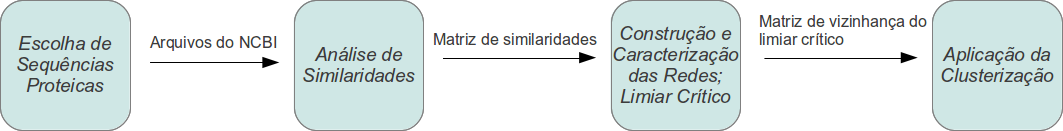
\includegraphics[scale=0.43]{fluxograma}
\caption{Fluxograma com os passos da execução do método de análise filogenética desenvolvido pelo FESC.}
\label{fig:fluxograma}
\end{figure}


\section{Escolha de Sequências Proteicas} \label{sec:escseq}

A primeira etapa do método consiste na escolha das sequências que serão utilizadas para a construção e caracterização da rede.
Usualmente a escolha é feita a partir de um banco de dados biológico, disponível livremente na \textit{web}. Durante o trabalho que necessitou da utilização
do método, as sequências escolhidas vieram do NCBI (\textit{National Center for Biotechnology Information}) \cite{ncbi},
um banco de dados bastante utilizado no
meio biológico, que contém dados de sequências
nucleotídicas e sequências proteicas, entre várias outras informações. A escolha das sequências proteicas é feita utilizando como critério
uma rota metabólica, separando as sequências pela enzima que as produzem na rota.

\sigla{NCBI}{\textit{National Center for Biotechnology Information}}

Esta é uma etapa manual, onde são feitas buscas por data e são realizadas determinadas filtragens no site do NCBI para obter as sequências desejadas, 
resultando em arquivos em um formato chamado GenBank. Um requisito importante para o sistema é a capacidade de receber um ou mais arquivos neste formato e
a partir deles
realizar uma filtragem e gerar a matriz de similaridades. O sistema deve levar em consideração que as sequências já foram escolhidas
e as receber como entrada inicial. O resultado desta etapa devem ser arquivos filtrados e organizados para facilitar a identificação de organismos em etapas
posteriores e proporcionar a execução da similaridade.

\section{Análise de Similaridades} \label{sec:similaridade}

Uma vez selecionadas as sequências, o próximo passo é executar a análise de similaridades entre as sequências proteicas e o armazenamento em um banco
de dados relacional. Para isso é utilizada a ferramenta BLAST (\textit{Basic Alignment Search Tool}) \cite{blast1997} para comparação entre as sequências.
A BLAST
trabalha tanto com sequências nucleotídicas quanto proteicas. O interesse do uso da BLAST para o método em questão está na comparação de sequências proteicas
utilizando o alinhamento local, que compara duas sequências isoladamente e retorna uma porcentagem de similaridade entre elas.

\sigla{BLAST}{\textit{Basic Alignment Search Tool}}

A capacidade de operar com a BLAST é um requisito de grande importância neste contexto, tanto no envio das sequências para comparação quanto no recebimento
e tratamento de seus resultados. A partir deles, pode-se construir uma matriz de similaridades \cite{andrade2011}, onde as linhas e colunas representam as
sequências e uma posição $(i, j)$ da matriz armazena a similaridade entre elas. Desta matriz são construídas as redes que caracterizam as sequências, que
serão descritas na próxima Seção.

\section{Construção e Caracterização das Redes} \label{sec:conscarac}

O conceito de rede está associado ao de um grafo, que é um par $G = (V, E)$ de conjuntos onde $E \subseteq [V]^2$, então os elementos de $E$
são subconjuntos de dois elementos de $V$. Para evitar ambiguidades de notação, devemos assumir que $V \cap E = \O{}$. Os elementos de $V$ são os vértices
(ou nós ou pontos) e os elementos de $E$ são suas arestas (ou linhas) \cite{reinhard2010}.

Podemos dizer que o estudo de uma rede é o estudo de um grafo, mas em uma escala maior. Redes podem ser tidas como grafos muito grandes e complexos,
onde se torna necessário o uso de técnicas estatísticas para a sua análise \cite{bessa2008}. Na literatura de Redes Complexas, em geral, precisamos
encontrar uma rede de determinado conjunto que melhor o caracterize. Essa escolha se dá pela relação entre ruído e informação \cite{barabasi2004}.

Partindo da matriz de similaridades, podemos construir até 101 matrizes de adjacência, relacionando cada matriz a uma escala de similaridade
de 0\% a 100\%, se levarmos
em consideração que podemos escolher um valor limiar e construir a rede baseada nele. Por exemplo, se escolhermos o valor 60 como limiar, construiremos uma
rede onde haverá uma aresta entre dois vértices (sequências) se e somente se a similaridade entre eles for maior ou igual a 60. Uma rede com limiar
muito baixo apresenta muito ruído, ou seja, muitas arestas, o que leva a pouca possibilidade de identificação de suas características. Por outro lado, uma
rede com limiar muito alto apresenta pouca informação, ou seja, poucas arestas, levando também a pouca possibilidade de identificação de suas características.

Partindo das matrizes de adjacência podemos também criar matrizes de vizinhança \cite{andrade2009}, que podem ser obtidas calculando-se os caminhos mínimos
\cite{bessa2008} entre os vértices da rede ou através da multiplicação booleana de matrizes de adjacência de ordens consecutivas \cite{andrade2006}. Na Figura 
\ref{fig:matriz-vizinhanca}, temos um exemplo de matriz de vizinhança, onde cada cor representa um valor de distância entre dois vértices. Pela Figura, temos
que se a distância entre dois vértices é 1, o ponto que representa a relação entre eles recebe a cor azul escura. Se for 7, por exemplo, receberá a cor
amarela.

Alguns programas utilizados geram as matrizes em memória e as excluem após determinados cálculos, e outros simplesmente as salvam em certa estrutura
de diretórios. A possibilidade de dar ao usuário o poder de gerenciar essas matrizes e realizar operações diversas, como compará-las ou visualizar gráficos
a partir delas ao longo de um procedimento de análise é algo importante que deve estar incluído em um ambiente integrado de análise filogenética.

\begin{figure}
\centering
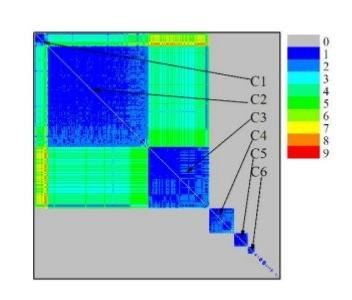
\includegraphics[scale=0.53]{matriz-vizinhanca}
\caption{Exemplo de Matriz de Vizinhança no formato de Matriz de Cores.}
\label{fig:matriz-vizinhanca}
\end{figure}

\section{Determinação do Limiar Crítico} \label{sec:limcrit}

Já se sabe que o limiar crítico de uma rede revela a melhor relação entre ruído e informação. Existem diversas maneiras de determiná-lo.
Uma delas é o método das distâncias \cite{andrade2009}. Nele, calcula-se a distância euclidiana entre matrizes de
vizinhança de limiares consecutivos \cite{andrade2011}. A matriz que apresentar a maior distância entre a matriz de limiar consecutivo
ao seu será a escolhida como a matriz do limiar crítico, para representar a rede. A literatura relacionada a Redes Complexas mostra que é necessário
escolher a melhor rede que representa o conjunto.
A rede do limiar crítico cumpre bem este papel.

Na Figura \ref{fig:distancia}, temos um exemplo de resultado do cálculo das distâncias entre matrizes de vizinhança, onde o limiar crítico é representado
pelo pico do gráfico, ou seja, o valor 51. A rede que representa todo o conjunto é então a rede limiar 51, que será utilizada na última etapa do processo:
a clusterização.

O método das distâncias pode ser utilizado para a determinação do limiar crítico, mas isto pode ser feito através de outros métodos, como a verificação da
variação do tamanho do maior \textit{cluster} da rede em função da variação do limiar. Portanto, um ambiente integrado deve fornecer a possibilidade de
escolha do método de análise dos limiares.

\begin{figure}
\centering
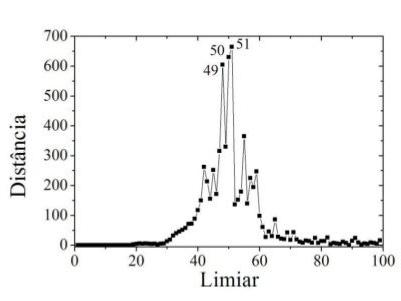
\includegraphics[scale=0.58]{distancia}
\caption{Resultado da execução do método das distâncias entre limiares consecutivos, resultando em um gráfico Distância x Limiar.}
\label{fig:distancia}
\end{figure}

\section{Entremeação} \label{sec:entremeacao}

A matriz de vizinhança da rede do limiar crítico é a entrada necessária para a realização da clusterização, que é feita através do método de detecção
de comunidades de Newman e Girvan \cite{newman2004} para identificar a estrutura modular da rede. O método consiste em determinar a aresta mais importante
da rede – aquela por onde passa a maior quantidade de caminhos mínimos de cada par de vértices por toda a rede – e eliminá-la, repetindo a operação
até que não existam mais arestas na rede. Estas operações consistem no conceito de \textit{Betweenness} ou Entremeação \cite{andrade2008}.

Conforme esta operação é feita, é possível construir um histograma de remoção de arestas ou dendrograma, que começa com uma linha representando toda a rede
e à medida em que as arestas são removidas a rede vai se repartindo em módulos e a linha inicial vai sofrendo bifurcações. Observando a Figura
\ref{fig:dendrograma}, por exemplo, entre o vértice 100 e 120 há uma bifurcação, indicando a divisão de um módulo em dois.

O dendrograma auxilia na identificação de comunidades (módulos) e propicia as análises biológicas dos resultados, além da comparação com outros
métodos da Biologia, visto que seu formato de árvore em que as linhas mais à direita representam cada uma das sequências proteicas (vértices da rede)
é também o formato de saída dos outros métodos de Análise Filogenética. 

Para a geração do dendrograma é necessária a escolha do limiar pelo usuário, e seu algoritmo recebe como entrada a matriz de vizinhança referente a este
limiar. A execução desta etapa é a mais demorada, variando de cinco minutos a mais de três meses, a depender do
tamanho da rede. 

\begin{figure}
\centering
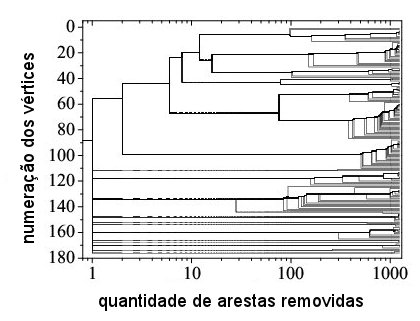
\includegraphics[scale=0.73]{dendrograma}
\caption{Exemplo de dendrograma para o limiar crítico 51.}
\label{fig:dendrograma}
\end{figure}

O método completo em questão é explicado com mais detalhes em \cite{goesneto2010} e \cite{andrade2011}. Ele utiliza uma série de programas, cada um
seguindo padrões de entrada e saída e arquivos de conFiguração particulares. Tais características dificultam sua utilização por pesquisadores de outras
áreas que não Física ou Ciência da Computação, além de deixar a seu cargo a tarefa de localizar, distribuir e organizar os arquivos. Para otimizar
o processo, seria mais interessante que o seu gerenciamento fosse realizado por um ambiente de fácil utilização e que
mantivesse disponíveis as informações por meio de uma camada de persistência, deixando a questão da organização dos dados transparente para o
pesquisador.

\section{A Proposta} \label{sec:proposta}

Da forma como está estruturado atualmente, o processo de análise filogenética através de redes complexas pode ser resumido como uma série de execuções
de programas independentes entre si que recebem arquivos
de entrada em determinados formatos, realizam seu
processamento e geram outros arquivos de saída. Os requisitos mais importantes, portanto, são a eliminação da necessidade de organização de arquivos
intermediários pelos usuários e a conversão de formatos entre as execuções. Para agilizar a execução, é importante também a geração de gráficos em
determinadas etapas. A tabela \ref{tab:requisitos} mostra de forma consolidada os requisitos levantados e que devem ser satisfeitos no processo de
modelagem e construção de um AIAF -
Ambiente Integrado de Análise Filogenética
Através de Redes Complexas.

\begin{table}
\centering
\caption{Tabela de requisitos do AIAF} % igual ao ambiente Figura
\begin{tabular}{p{5cm}p{10cm}} % com este comando dizemos quantas colunas terá nossa tabela e a posição do texto dentro de cada coluna. Aqui temos três colunas (pois são três "c" dentre {}) e o texto estará centralizado em todas elas (indicado pelo "c", se quisermos alinhados à esquerda "l" ou direita "r"
\hline 
%Requisito & Pontos & Classificação \\
Requisito & Descrição \\ 
\hline
\hline
%Cruzeiro & 52 & 1 \\
%Sao Paulo & 50 & 2 \\
%Gremio Barueri & 47 & 3 \\
Filtragem de arquivos no formato GenBank & O sistema deve receber um diretório e ler dele arquivos no formato do GenBank, e a partir deles criar os
organismos, as sequências com nome, identificador, código e outras informações\\ \hline
Controle da análise & O sistema deve prover ao usuário a possibilidade de criar, salvar ou carregar uma análise \\ \hline
Salvamento de organismos e sequências & O sistema deve salvar os organismos e as sequências para posterior consulta. Deve ser criada uma estrutura de
armazenamento que livre o usuário da necessidade de instalar sistemas de bancos de dados relacionais \\ \hline
Escolha de sequências & O sistema deve permitir a escolha de sequências para a geração da matriz de similaridades \\ \hline
Geração de matrizes de adjacência & O sistema deve gerar matrizes de adjacência com base no limiar fornecido pelo usuário, também mostrando o gráfico de uma
forma opcional \\ \hline
Geração de matrizes de vizinhança & O sistema deve gerar matrizes de vizinhança com base no limiar fornecido pelo usuário, também mostrando o gráfico de uma
forma opcional \\ \hline
Análise de limiares & O sistema deve fornecer opções de métodos para a análise de limiares, mostrando obrigatoriamente o gráfico como resultado\\ \hline
Execução da clusterização & O sistema deve fornecer opções de métodos de clusterização, que depende da escolha de um limiar pelo usuário, além de mostrar
o gráfico de seu resultado quando requisitado \\ \hline
Visualização do gráfico completo da rede & O sistema deve permitir a visualização do gráfico completo da rede, após a escolha das comunidades,
recuperando as informações salvas durante o processo de salvamento das sequências e organismos \\ \hline
Congruência & O sistema deve permitir a comparação do resultado do método com o resultado de outros métodos de análise filogenética, além da comparação
com o resultado pelo próprio método com outro conjunto de dados \\ \hline
Exportação de dados & O sistema deve permitir a exportação de dados necessários à geração de gráficos para o uso pelos usuários de ferramentas
profissionais de plotagem \\ \hline
\end{tabular}
\label{tab:requisitos}
\end{table} 

A partir desses requisitos gerais, apresentamos no próximo Capítulo a proposta de modelagem que pretende atendê-los.


\chapter{Modelagem do AIAF - Ambiente Integrado de apoio à Análise Filogenética através de Redes Complexas}
\label{cap:navi}

\sigla{AIAF}{Ambiente Integrado de apoio à Análise Filogenética através de Redes Complexas}

A partir dos requisitos identificados no Capítulo anterior, podemos propor um ambiente integrado para gerenciar o método de Análise Filogenética por
Redes Complexas descrito anteriormente. Para garantir o controle das etapas do processo e ao mesmo tempo permitir uma fácil utilização e evitar problemas
com padrões e arquivos de conFiguração, o sistema precisa seguir três importantes pilares:

\begin{itemize}
 \item{\textbf{Usabilidade:} é um fator importante por tornar o método passível de utilização por pessoas com pouco ou quase nenhum conhecimento de
programação neste caso específico, e para gerar uma boa experiência do usuário e fazer com que seu uso seja agradável no caso geral. Segundo
\cite{nielsen1993}, interfaces de usuário são uma parte muito mais importante para computadores em geral do que já foram um dia, e hoje respondem por mais
de 45\% do código-fonte de um \textit{software}. Podemos também enquadrar aqui as interfaces de programação, levando a uma fácil manutenção e possibilitando
extensibilidade.}
  \item{\textbf{Gerenciamento da Informação:} torna possível a criação, importação e exportação de dados contendo as execuções necessárias para as análises,
onde os dados podem ser agrupados em um formato de arquivo possível de ser transportado entre múltiplas máquinas e contendo todas as informações
necessárias para a retomada de execuções.}
  \item{\textbf{Transparência:} não menos importante, permite que as pessoas que estão executando o método não precisem se
preocupar com detalhes de mais baixo nível de execução, como os locais em que os arquivos estão dispostos e situações relacionadas à conversão de
formatos e adaptações diversas de dados.}
\end{itemize}

Para satisfazer a todos os requisitos e possuir as características citadas acima, este trabalho seguiu uma metodologia tradicional de projetos
de Engenharia de Software \cite{softeng2005} e foi adotado o modelo de desenvolvimento em espiral, onde há ciclos de planejamento de requisitos,
com concepção de requisitos, criação
de um protótipo, verificação, validação e novo planejamento de requisitos, continuando o ciclo \cite{boehm1986}. Neste trabalho apenas uma
parte da espiral foi percorrida.

No levantamento de requisitos, foram determinados os objetivos e alternativas e definido o escopo do sistema baseado nos objetivos do projeto,
dispostos na Seção \ref{sec:objetivos}. Em seguida foi realizada a modelagem, com os diagramas de casos de uso, classes e sequência.
Também foi definida a forma como o sistema organizaria e realizaria a persistência de seus dados, levando em consideração os requisitos definidos.
A última etapa do primeiro ciclo da espiral consistiu no planejamento do desenvolvimento, implementação do protótipo e testes.

Este Capítulo trata das etapas de modelagem, que foram realizadas utilizando a linguagem UML \cite{uml}. A implementação do protótipo e os testes são
tratados no Capítulo 4.

\section{Casos de Uso} \label{sec:escopo}

Esta seção discute os casos de uso do AIAF, que podem ser vistos na Figura \ref{fig:casos-uso}.

\begin{figure}
\centering
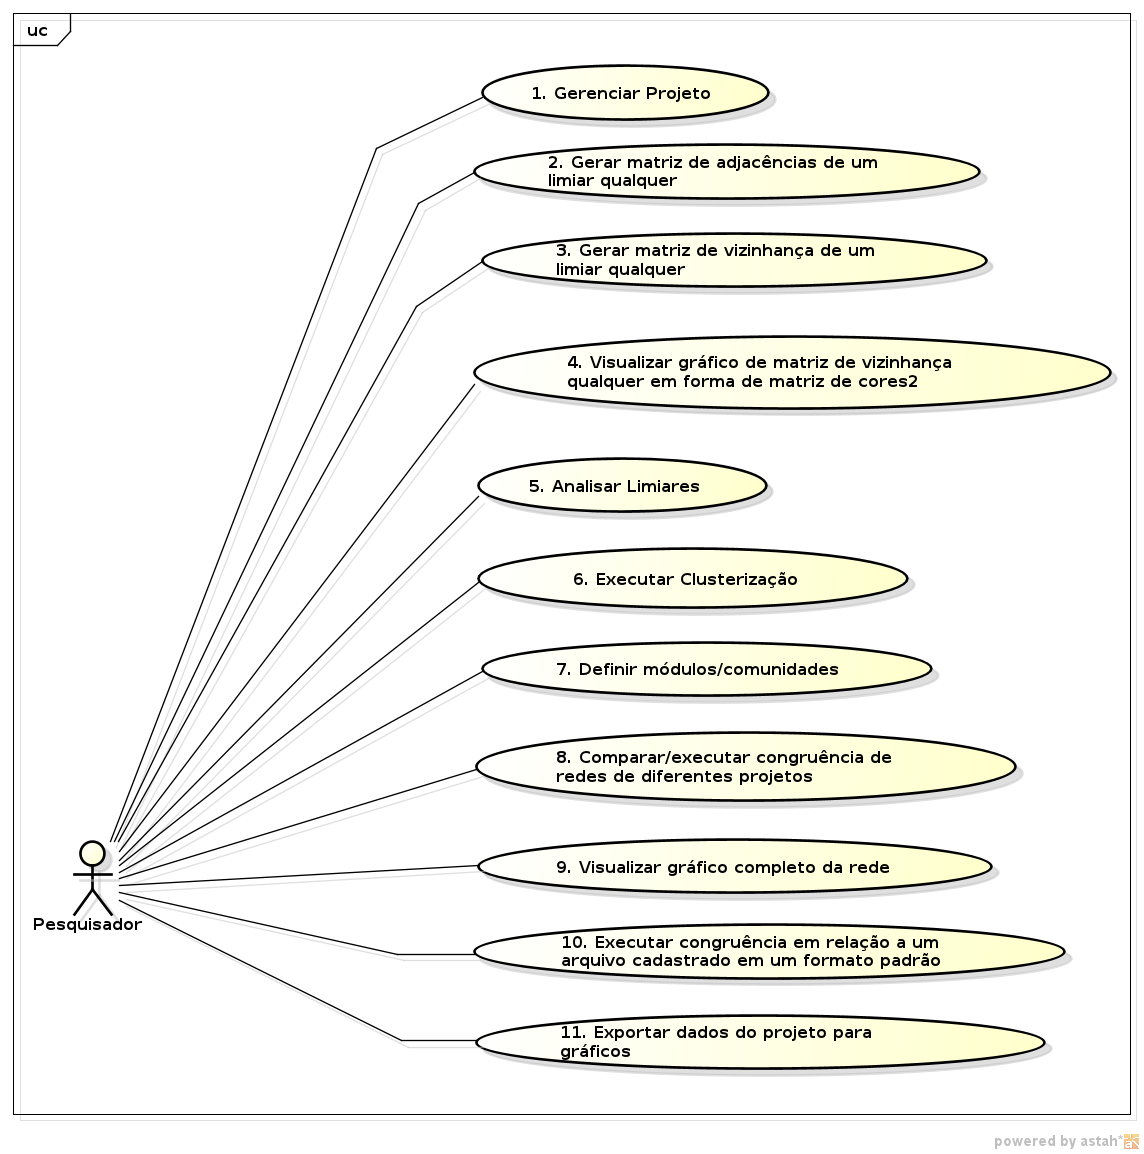
\includegraphics[scale=0.52]{diagrama-casos-de-uso}
\caption{Diagrama de casos de uso do AIAF.}
\label{fig:casos-uso}
\end{figure}

O processo de análise atual utiliza um banco de dados relacional para armazenamento de informações
sobre as sequências proteicas. Isto força o usuário a instalar
um banco de dados e configurá-lo corretamente. Um dos requisitos importantes, como visto no Capítulo anterior, é a retirada desta necessidade e,
por consequência, a criação de uma nova forma de organização e disposição dos dados.

Diversos ambientes de \textit{software} trabalham com o conceito de projeto. Um projeto
representa um conjunto de operações feitas durante a execução do sistema,
podendo-se salvar e recuperar o andamento das atividades. Tal fato é possível a partir de uma estruturação de dados para um correto procedimento de
salvamento e posterior recuperação das informações. Trabalhar com projeto se torna importante na medida em que se pode
dar ao usuário a possibilidade de criar
diversas análises, importar seus resultados e armazenar suas informações em qualquer etapa do processo.
Isto permite uma interoperabilidade entre máquinas importante, e a organização de um arquivo
que possa conter os dados necessários para o carregamento de um projeto salvo torna-se essencial. O sistema então permitirá aos seus usuários a criação de
novos projetos e o carregamento de projetos existentes (casos de uso 1 e 2).

A comunicação com módulos externos deve ser transparente e a organização de classes deve fornecer alternativas viáveis para a inclusão de novos
tipos de análises, como por exemplo, a escolha do limiar crítico pode ser feita por uma análise de distâncias, como também por uma análise da variação
do tamanho
do maior \textit{cluster} da rede, ou seja, o sistema deve suportar extensibilidade e a fácil troca de módulos externos, mantendo
os padrões de comunicação.

A partir de certo momento do processo, passa-se a trabalhar apenas com matrizes. Há a perda de informações com relação aos organismos e sequências em que
se está trabalhando. É necessário, então, que o sistema guarde estas informações e possa exibir para os usuários gráficos mais ricos, contendo informações
sobre sequências e espécies com que se está trabalhando. Por exemplo, na exibição da rede (grafo), o sistema poderia exibir, ao se passar o mouse sobre um
vértice,
informações sobre a sequência e o organismo a que o vértice está representando (caso de uso 10). O usuário poderá também gerar matrizes de adjacência e
vizinhança a qualquer momento (casos de uso 3 e 4), além de ver o gráfico de qualquer matriz de vizinhança em formato de matriz de cores (caso de uso 5).

Em várias etapas da execução do processo de análise atual, é necessário mudar de ambiente (tipicamente, de Linux para Windows) para efetuar certo processamento,
como por exemplo visualizar
gráficos em
programas específicos \cite{origin},
que são necessários para certas tomadas de decisões que influenciam em quais dados serão escolhidos para a execução das próximas etapas do mesmo. Isto é
prejudicial pois gera uma troca de contexto. O sistema, então, pode gerar esses gráficos (matrizes de vizinhança em forma de matrizes de cores, matrizes de
adjacências em forma de grafos, gráficos de resultados de análises como distâncias, gráfico do dengrograma), mesmo que com qualidade um pouco inferior,
para que a continuação do processo se dê de forma mais rápida. Esta funcionalidade representa
uma preocupação que deve estar presente no momento da modelagem para
tornar o processo mais ágil e transparente para o usuário. Ao mesmo tempo, o sistema pode fornecer como opção de exportação os arquivos que são utilizados por
programas profissionais de plotagem, essenciais para a utilização em artigos científicos e afins (caso de uso 12).

A análise de limiares (caso de uso 6) resulta na geração de um gráfico que será utilizado como base para a definição do limiar crítico e o prosseguimento
do processo, com a clusterização (caso de uso 7) e a definição de comunidades (caso de uso 8).

Outro detalhe importante é a possibilidade de comparação entre o método atual desenvolvido pelo FESC
e outros métodos já consolidados de análise filogenética, listados no Capítulo \ref{cap:analisefilo},
além de poder comparar com outro projeto criado pelo próprio sistema (casos de uso 9 e 11).
Para prosseguir com a modelagem, se faz necessária a organização das informações através
de um diagrama de classes, mostrado na próxima Seção.

\section{Modelagem dos Dados} \label{sec:organizacao}

A organização das informações do sistema é um passo importante para que se tenha qualidade e se atenda aos requisitos propostos. Por conta da metodologia
adotada, é imprescindível a criação de um diagrama de classes para definir classes e suas responsabilidades, além de seus aspectos funcionais (métodos)
e os dados
(atributos) em que cada uma é responsável.

Após análise das informações manipuladas no ambiente de análise atual e considerando os casos de uso definidos na Seção anterior,
foi criado um diagrama de classes, cuja versão simplificada pode ser vista na Figura
\ref{fig:diagrama-classes-simplificado}. O diagrama de classes completo pode ser encontrado no Apêndice A.

\begin{figure}
\centering
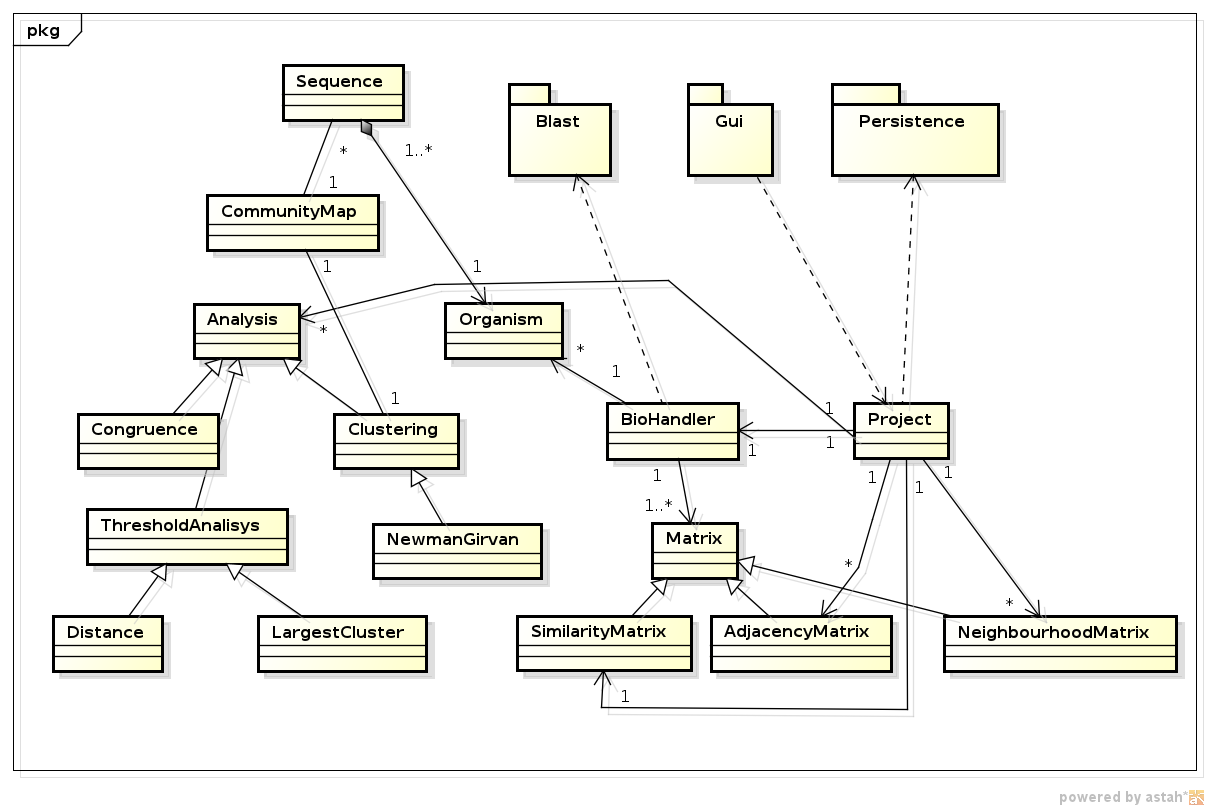
\includegraphics[scale=0.52]{diagrama-classes-simplificado}
\caption{Diagrama de classes simplificado do AIAF.}
\label{fig:diagrama-classes-simplificado}
\end{figure}

A classe principal do AIAF é a classe \textit{Project}. Todas as interações do usuário com a \textit{GUI} passam por ela, que controlará operações com
matrizes, análises, tratamento das informações biológicas e dos dados de entrada. Através dela é possível criar novo projeto, abrir projeto existente e
salvar projeto corrente (casos de uso 1 e 2). Um projeto para o sistema reúne todos os dados de informações de execução de um conjunto de dados, desde
a escolha de sequências, geração de matriz de similaridade, matrizes de adjacência e vizinhança, gráficos, definição de comunidades, clusterização,
congruência. A classe \textit{Project} também lida com o pacote \textit{Persistence}, que mapeia as classes do sistema em uma camada de persistência, via
armazenamento em disco. Sua função inclui serializar e desserializar os objetos do sistema, além de prover
a organização dos dados do projeto, atuando de forma transparente ao usuário. Como resultado, o usuário obtém um arquivo que representa o mapeamento
feito pela camada de persistência em um sistema de arquivos comprimido e de extensão própria (.aiaf).

\sigla{GUI}{\textit{Graphical User Interface}}

A filtragem do banco de dados biológico (sequências proteicas que estão em vários arquivos no diretório especificado pelo usuário) é realizada pela classe
\textit{BioHandler}, que a partir desta operação instancia objetos da classe \textit{Organism} e da classe \textit{Sequence}, ou seja, cria organismo e associa
sequências a eles. Neste contexto, um organismo pode conter uma ou mais sequências, o que explica a composição realizada no diagrama de classes.
Ela utiliza o pacote \textit{Blast}, que realiza as comparações entre sequências, para gerar e instanciar a matriz de similaridades.

O AIAF possui três matrizes, representadas pelas classes \textit{SimilarityMatrix}, \textit{AdjacencyMatrix} e \textit{NeighbourhoodMatrix}. As três herdam
da classe \textit{Matrix} por conterem características em comum. Só é possível ter uma matriz de similaridades por projeto, pois como um projeto está associado
a execuções de determinado conjunto de sequências escolhido pelo usuário, há apenas uma matriz de similaridades possível para qualquer conjunto de sequências.
Em relação às demais (adjacência e vizinhança), é possível haver mais de uma. Outros tipo de matrizes poderão ser
facilmente incorporadas ao sistema através da adição de uma nova classe que será uma especialização da classe \textit{Matrix}, o que explica o fato de a classe
\textit{Matrix} ser um classe abstrata. É possível gerar matrizes de adjacência ou de vizinhança, além da visualização de seus respectivos gráficos a qualquer
momento após a escolha das sequências e geração da matriz de similaridades, de acordo com os casos de uso 3, 4 e 5. A classe \textit{Project} contém métodos
para a geração das matrizes, o que pode ser visto no diagrama de classes completo no Apêndice A.
Após a geração das matrizes, a camada de persistência as salva em disco de forma transparente.

A classe \textit{Analysis} é uma classe abstrata que concentra todos os tipos de análises que podem ser feitas sobre as matrizes relacionadas às redes
proteicas. Existem três tipos de análises: Análise de Limiares (classe \textit{ThresholdAnalysis}), Clusterização (classe \textit{Clustering}) e
Congruência (class \textit{Congruence}). Como descrito anteriormente, existem duas formas atualmente de analisar limiares: Distâncias (classe
\textit{Distance}) e tamanho do maior cluster (classe \textit{LargestCluster}). Elas são subclasses de \textit{ThresholdAnalysis}, que também é abstrata. Essa
abordagem permite que outros métodos de análise de limiares possam ser adicionados de forma facilitada por meio de herança. O mesmo acontece com a
clusterização: a classe \textit{Clustering} é abstrata, e tem \textit{NewmanGirvan} como classe filha, que implementa o único método de clusterização
usado no processo até o momento (casos de uso 6 e 7).

A análise de congruência permite a comparação da divisão de comunidades entre diversos projetos executados sob o AIAF, como também entre outros métodos de
análise filogenética, através do fornecimento de um arquivo em formato padrão. Isso é possível graças à classe \textit{Congruence}, que é uma
especialização da classe
\textit{Analysis} (casos de uso 8 e 10).

Outras funcionalidades do sistema incluem a visualização do gráfico completo da rede, que utiliza a classe \textit{CommunityMap} para desenhar
os vértices que pertencem a uma mesma comunidade de determinada cor (caso de uso 9); e a possibilidade de exportar dados do projeto para
gráficos em um formato de programas plotadores, utilizando-se de atributos de diversas classes, a depender do gráfico que se deseja (caso de uso 11).

O diagrama de classes permite ter uma visão estática das informações do sistema, enfatizando os seus relacionamentos e os métodos que as irão manipular.
Na próxima Seção serão apresentados e discutidos os principais diagramas de sequência, que fornecem uma visão dinâmica da interação entre as diversas
classes do modelo ao longo do tempo.

\section{Diagramas de Sequência} \label{sec:dinamica}

Como discutido na Seção anterior, a classe \textit{Project} é a classe principal do sistema, para onde os eventos captados pela interface gráfica são
enviados. Nesta Seção serão abordados três importantes diagramas de sequência do AIAF: criar novo projeto, gerar matriz de adjacência de um limiar qualquer
e analisar limiares. Os casos de uso 2, 5, 7, 8, 9, 10, 11 e 12 são autoexplicativos, e o caso de uso 4 é análogo ao caso de uso 3. Será
apresentada uma discussão sobre sua dinâmica. Outros diagramas de sequência podem ser encontrados no Apêndice B - Anexo II.

O primeiro diagrama de sequência, visto na Figura \ref{fig:new-project}, se refere à criação de um novo projeto (caso de uso 1). Primeiro, qualquer projeto
que esteja em execução é finalizado e o pacote \textit{Persistence} salva qualquer alteração nos objetos do sistema. Uma decisão de projeto importante
é que após a instanciação de uma nova classe \textit{Project} é criado também um novo objeto \textit{BioHandler}, que já filtra os dados passados pelo
usuário, criando objetos \textit{Organism} e \textit{Sequence}. Após isto, \textit{Persistence} salva os dados do projeto.

Em seguida o usuário escolherá as sequências com que a matriz de similaridades será gerada, onde \textit{BioHandler} passará as sequências, duas a duas,
para que o pacote \textit{Blast} possa calcular as porcentagens, e então o primeiro possa montar a matriz de similaridades. Por fim, os dados do projeto
são salvos em disco pela classe de persistência.

\begin{figure}
\centering
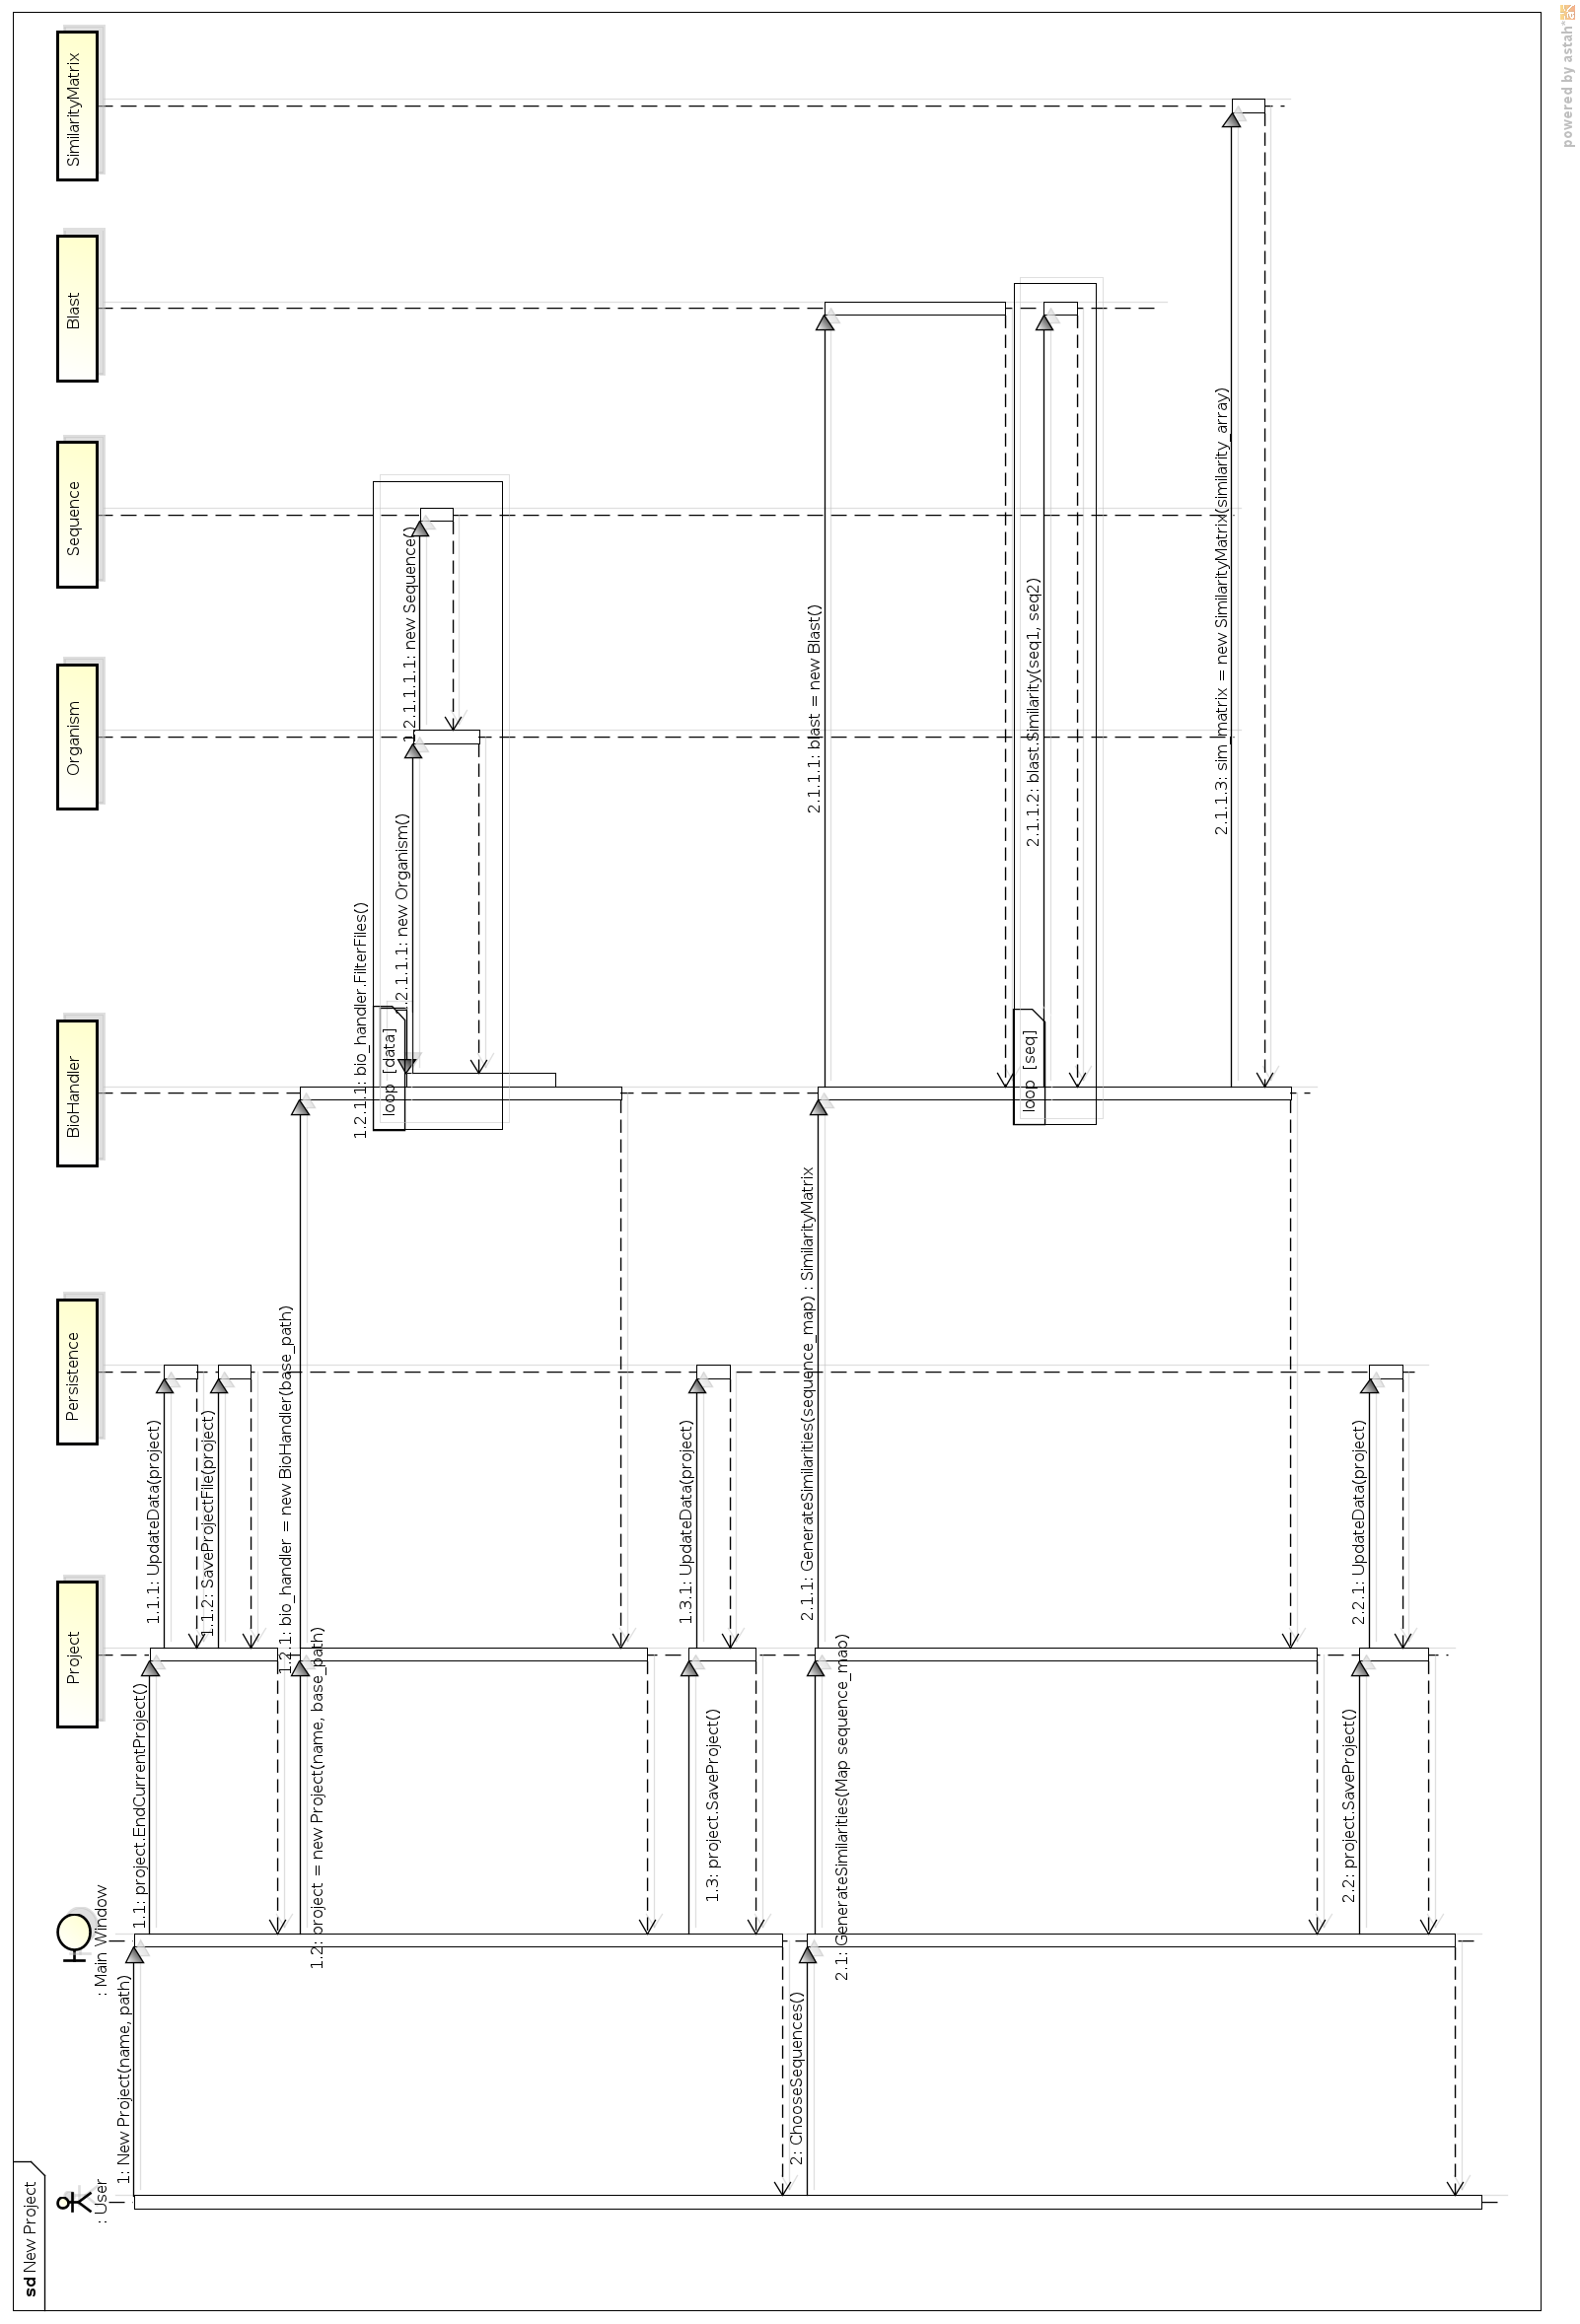
\includegraphics[scale=0.27]{new-project}
\caption{Diagrama de sequências para o caso de uso 1: criar novo projeto.}
\label{fig:new-project}
\end{figure}

Para gerar uma matriz de adjacências (caso de uso 3)
o usuário entra com um valor limiar (ou uma lista de limiares para o caso da geração de múltiplas matrizes). Haverá
então um \textit{loop} na classe \textit{Project} que instanciará objetos da classe \textit{AdjacencyMatrix}, e então usará \textit{Persistence} para salvar
novos dados em disco, conforme a Figura \ref{fig:generate-adjacency-matrix}.

\begin{figure}
\centering
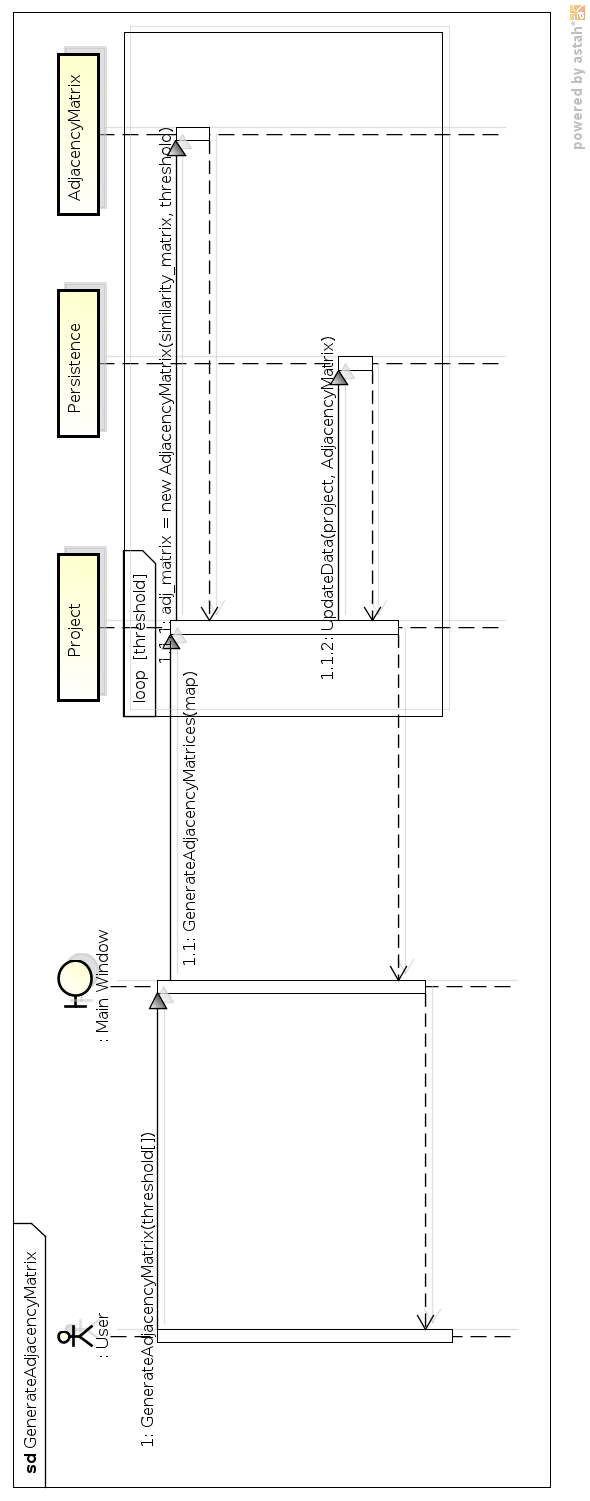
\includegraphics[scale=0.42]{generate-adjacency-matrix}
\caption{Diagrama de sequências para o caso de uso 3: gerar matriz de adjacências de um limiar qualquer.}
\label{fig:generate-adjacency-matrix}
\end{figure}

Para analisar limiares (caso de uso 6),
o usuário precisa informar qual análise quer executar. O método do FESC de análise filogenética dispõe atualmente de duas formas
para a realização desta análise, mas existem vários outros e que podem ser adicionados ao AIAF. Atualmente o usuário deve optar, então, pelo método de
distâncias ou tamanho do maior cluster. A depender da escolha será instanciado pela classe \textit{Project} uma classe \textit{Distance} ou
\textit{LargestCluster}. A análise é realizada passando-se a matriz de similaridades e, ao seu final, é invocada uma biblioteca gráfica
para a exibição do gráfico para o usuário como resultado da análise. A Figura \ref{fig:analyse-threshold} mostra seu diagrama de sequência.

\begin{figure}
\centering
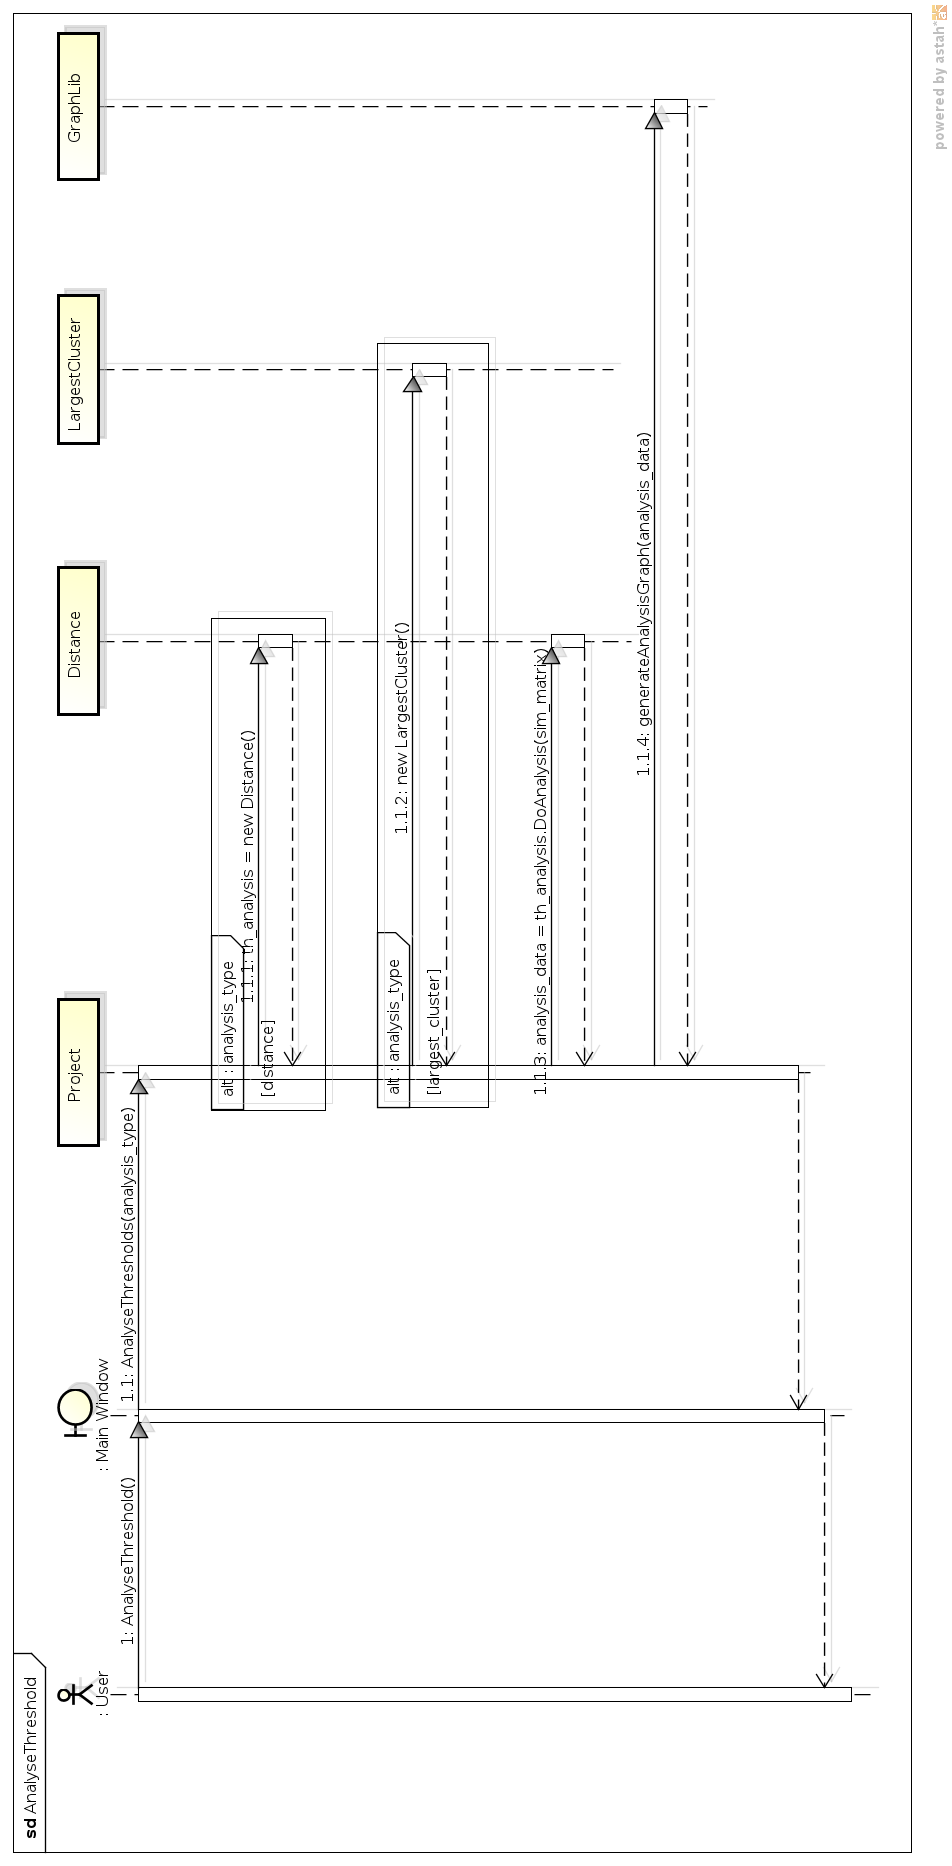
\includegraphics[scale=0.34]{analyse-threshold}
\caption{Diagrama de sequências para o caso de uso 6: analisar limiares.}
\label{fig:analyse-threshold}
\end{figure}

O próximo Capítulo mostrará os resultados deste trabalho, seu produto gerado, as ferramentas e o ambiente de execução utilizados, características
de implementação e discutirá os resultados em relação aos objetivos propostos pelo trabalho.

\chapter{Resultados Obtidos}
\label{cap:resultados}

Neste Capítulo são apresentadas de forma detalhada as técnicas utilizadas para o desenvolvimento do AIAF.


\section{Ambiente de Desenvolvimento} \label{sec:ambiente}

O ambiente operacional original
envolve uma série de ferramentas e linguagens: exige um ambiente GNU/Linux, um compilador Fortran, um compilador C, pacotes para
a execução de \textit{scripts} Perl e a biblioteca \textit{BioPerl}, além de um banco de dados relacional, neste caso o MySQL. Após o \textit{download} das
sequências a partir do banco de dados GenBank, as mesmas eram colocadas em um mesmo diretório, onde uma série de \textit{scripts} Perl eram executados,
realizando os passos necessários para o armazenamento das sequências no banco de dados e a posterior geração da matriz de similaridades.

De posse da matriz de similaridades, é necessária a execução de outro programa para a geração das redes de diversos limiares e análise dos mesmos para que
fosse possível a escolha de um limiar crítico e então a continuação do método.
Utilizando então a matriz de vizinhança da rede do limiar crítico, a clusterização é aplicada, gerando como
resultado um dendrograma (histograma de remoção de arestas, indicando modularização da rede). O dendrograma, em conjunto com a matriz de cores e as sequências
permitem análises biológicas sobre os resultados.

Os módulos permanecem os mesmos, mas o controle do processo é todo gerenciado pela GUI, a classe \textit{Project} e o pacote \textit{Persistence},
com auxílio de
outras classes na execução e comunicação dos módulos externos. A Seção \ref{sec:discussao} detalha como se dá este gerenciamento.

A área de Bioinformática hoje em dia tem utilizado bastante Python \cite{python} no lugar de Perl para comparações entre sequências, utilização de algoritmos
genéticos, entre outras técnicas na pesquisa em geral. É uma linguagem bastante rica e poderosa, com uma grande facilidade de uso, compreensão e
desenvolvimento, rapidez na implementação e na prototipagem, bibliotecas robustas para o desenvolvimento de \textit{software} científico, cálculos
diversos e geração de gráficos, além de ser considerada uma ``linguagem cola'' por se comunicar facilmente com outras linguagens.

Para a modelagem foi utilizado o Astah Community \cite{astah}. Para a criação das janelas foram testados o Tkinter (que vem com a linguagem Python), o Gtk
e o Qt. O Qt foi escolhido pela sua quantidade de recursos, facilidade de utilização, desenvolvimento e manutenção, total suporte à linguagem Python através
do PyQt \cite{pyqt}, além de fornecer o \textit{Designer}, um bom ambiente de autoria para a criação de janelas e interface gráfica em geral.
A utilização de Qt também permite a possibilidade de execução do AIAF em ambientes Windows e Mac,
faltando apenas a adaptação do \textit{back-end} para um suporte completo a essas outras plataformas.

A utilização da linguagem Python para o desenvolvimento do AIAF acarretou certas consequências. Uma delas foi a substituição do \textit{BioPerl} pelo
\textit{BioPython} \cite{biopython}, um conjunto de ferramentas para computação biológica feito em Python, equivalente ao \textit{BioPerl} para \textit{Perl}.
Um dos gargalos na execução do método original é também a necessidade de observar gráficos e a partir deles tomar decisões relativas ao prosseguimento do
processo. Como a execução dos diversos programas era feita em Linux e o programa plotador de gráficos, o Origin \cite{origin}, roda em Windows, em várias
situações era necessário reiniciar a máquina ou mudar de máquina para que se pudesser plotar os gráficos. Com o Matplotlib \cite{matplotlib}, biblioteca de 
plotagem de gráficos para Python, esse trabalho passa a ser desnecessário.

O \textit{BioPython} inclui o Blast2 e seus \textit{bindings} para Python. Como módulos externos, se fizeram necessários ainda o Madchar (geração de matrizes),
o RedeCrítica (análise de limiares) e o Dendo (clusterização). Por serem codificados em Fortran foi necessário o pacote Gfortran.

\section{Discussão} \label{sec:discussao}

A primeira preocupação na implementação do AIAF foi a questão inicial da filtragem e armazenamento dos dados. Um banco de dados relacional é uma exigência
muito grande para um sistema que vai realizar certos cálculos e gráficos, e que será utilizado em larga escala em máquinas diversas e por pesquisadores de
áreas como Biologia. Por isso, a primeira decisão foi a troca do banco de dados relacional por uma estrutura de armazenamento de dados através da serialização
de objetos, sendo útil também na criação de um projeto e o carregamento de um projeto existente no disco, que são atribuições do pacote 
\textit{Persistence}. Em sua versão atual, o protótipo do AIAF utiliza uma solução simples para a persistência, baseada no módulo \textit{Pickler} do
Python para a serialização de todos os objetos do sistema em um único arquivo.


Um arquivo .aiaf (extensão de arquivo do AIAF) é simplesmente um pacote compactado que contém uma estrutura de diretórios, destinada a armazenar os arquivos
necessários à execução de um projeto, e também fornece suporte a certas operações de execução. Quando necessário, o pacote \textit{Persistence} descompacta
o .aiaf em um diretório temporário, espera certas operações serem realizadas e então compacta novamente na localização original, utilizando a biblioteca
\textit{zipfile} do Python. Os processos de compactação e descompactação são transparentes para o restante da aplicação.

A filtragem feita originalmente não incluía uma opção de escolha das sequências com que se desejasse trabalhar, fazendo com que todas as sequências dos
arquivos do GenBank fossem utilizados na geração da matriz de similaridades. No AIAF, a criação de um novo projeto resulta
na filtragem e armazenamento dos dados, e em seguida a possibilidade de escolha das sequências, como mostra a Figura \ref{fig:choose-sequences}.

\begin{figure}
\centering
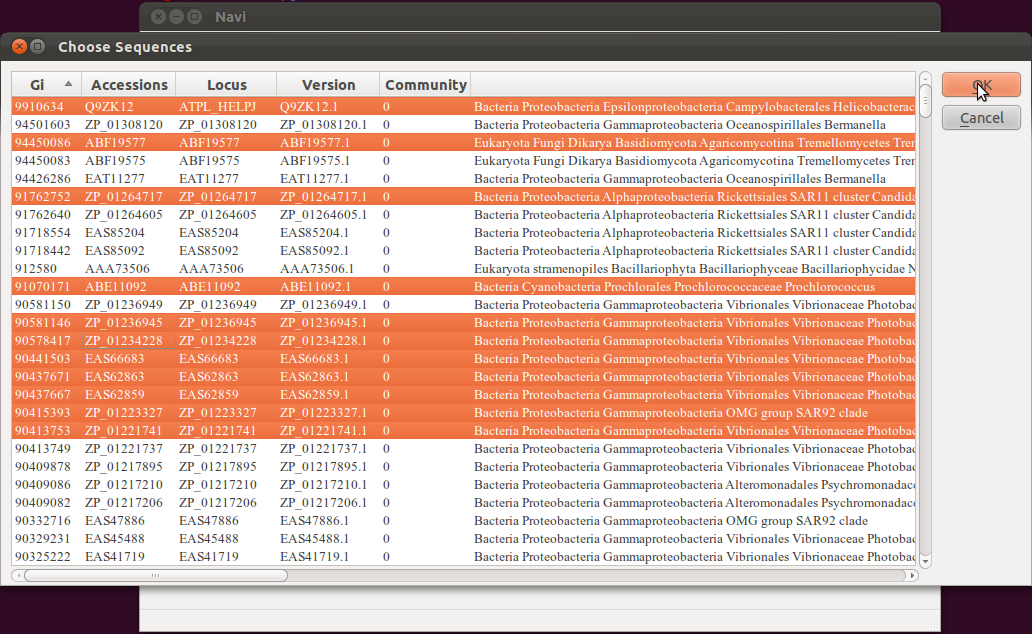
\includegraphics[scale=0.38]{choose-sequences}
\caption{Escolha das sequências no AIAF após filtragem.}
\label{fig:choose-sequences}
\end{figure}

A geração de matrizes de adjacência é feita na construção de um objeto da classe \textit{AdjacencyMatrix}, pela própria camada de negócio do AIAF, sem a
necessidade de invocar módulos externos, pela simplicidade da operação. Já para gerar as matrizes de vizinhança, o módulo Madchar é invocado. A operação
também é realizada durante a construção de um objeto da classe \textit{NeighbourhoodMatrix}, onde seu construtor invoca o método
\textit{generate\_neighbourhood\_values}. A Figura \ref{fig:generate-matrices} ilustra a interface de geração de matrizes.

\begin{figure}
\centering
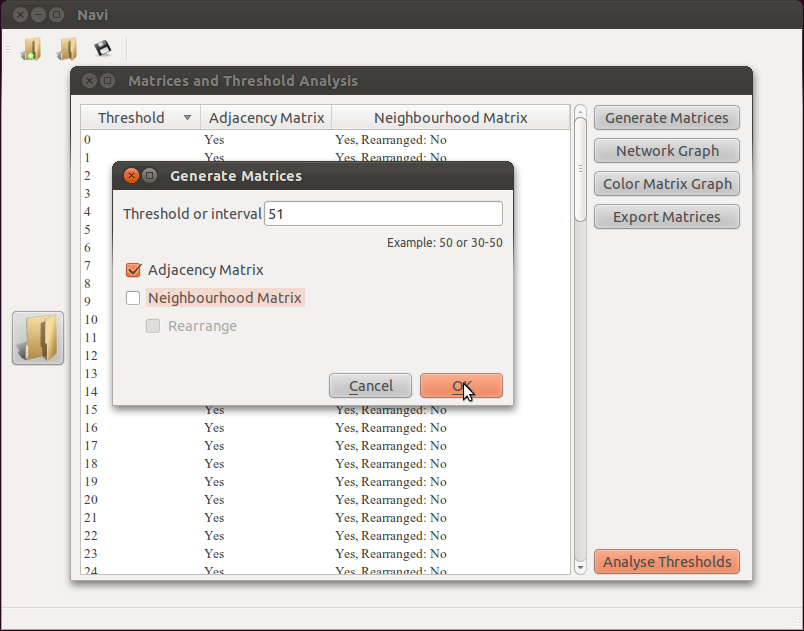
\includegraphics[scale=0.38]{generate-matrices}
\caption{Geração de matrizes no AIAF.}
\label{fig:generate-matrices}
\end{figure}

A visualização do gráfico de matriz de cores se baseia nos dados da matriz de vizinhança e simplesmente os utiliza como entrada para a biblioteca
\textit{Matplotlib} desenhar o gráfico na tela.

Como descrito na Seção \ref{sec:organizacao}, a classe \textit{Analysis} tem a \textit{ThresholdAnalysis} como subclasse,
que por sua vez tem como descendentes classes que representam as diferentes formas de execução da análise de limiares. Isso permite uma extensibilidade
ao AIAF, uma vez que basta acrescentar uma nova descendente à \textit{ThresholdAnalysis} para se incluir um novo método de analisar limiares. A situação
é análoga para a clusterização, com a classe \textit{Clustering} e sua filha \textit{NewmanGirvan}.

Nesta versão do protótipo do AIAF, apenas o método de distâncias foi implementado, por meio de invocação do módulo externo RedeCrítica por um método da
classe \textit{Distance}, que é filha da classe \textit{ThresholdAnalysis}. Para a clusterização, o método de Newman e Girvan foi implementado por meio
de invocação de um módulo externo feito em Fortran (Dendo). A invocação dos módulos Fortran foi feita utilizando chamadas de sistema da linguagem Python,
que não permite uma integração perfeita, mas se utiliza do poder da linguagem de mapear as chamadas de sistema para a plataforma em que o \textit{software}
está sendo executado. A Figura \ref{fig:clustering-gui} ilustra a interface com o usuário para a execução da clusterização e a Figura \ref{fig:navi-dendrogram}
ilustra o dendrograma, resultado final do método, gerado pelo AIAF.

A etapa de congruência foi modelada mas não foi implementada no protótipo pela dificuldade de implementação, pela necessidade de estudo profundo nos outros
métodos de análise filogenética e as ferramentas existentes para tal, além de adequar as saídas a um formato padrão para executar a comparação. Tal trabalho
exigiria mais tempo que o disponível. Mais informações sobre outros métodos e a congruência podem
ser vistas em \cite{marcelo2010}. Como o AIAF não é capaz de gerar gráficos tão bons quanto uma suíte profissional dedicada à plotagem destinada a artigos e
trabalhos científicos em geral, e há perda do controle do usuário sobre a localização e o formato dos dados gerados entre as diversas etapas do processo, se
faz necessária a exportação desses arquivos para que o usuário os utilize como fonte para utilização em programas plotadores.
Esta funcionalidade, no entanto, não foi implementada no protótipo.

Duas outras funcionalidades também não foram implementadas no protótipo, que são a definição de módulos/comunidades (caso de uso 8), onde o usuário define
com base na matriz de cores e no dengrograma quais sequências pertencem a quais comunidades e com isso pode ser gerado o gréfico completo da rede (caso de
uso 10) para visualização, onde o usuário pode ver as comunidades separadas por cores, além de obter facilmente informações sobre as sequências clicando nos
vértices. Estas funcionalidades em conjunto
exigem um trabalho de interface gráfica grande, incluindo a exibição interativa de gráficos e a integração de bibliotecas de exibição de
gráficos a bibliotecas de plotagem.

\begin{figure}
\centering
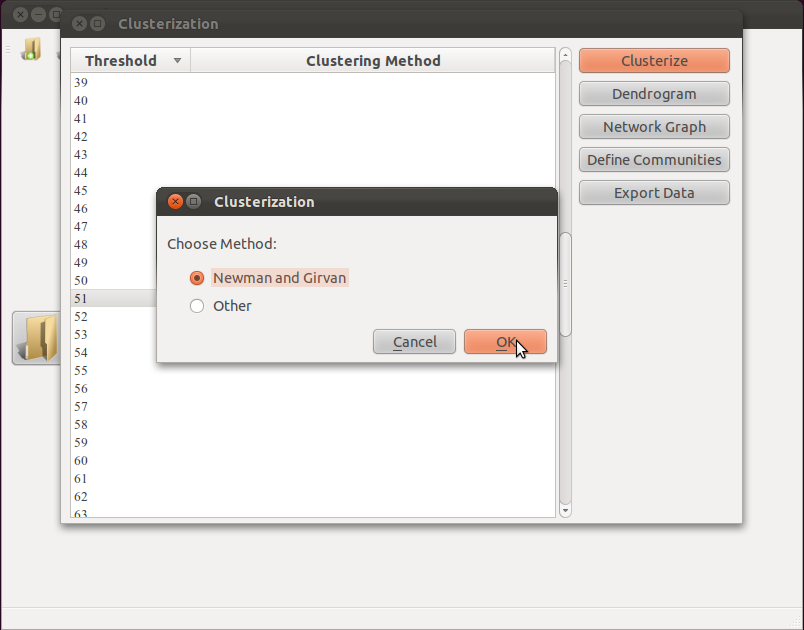
\includegraphics[scale=0.38]{clustering-gui}
\caption{Interface de execução da clusterização no AIAF.}
\label{fig:clustering-gui}
\end{figure}

\begin{figure}
\centering
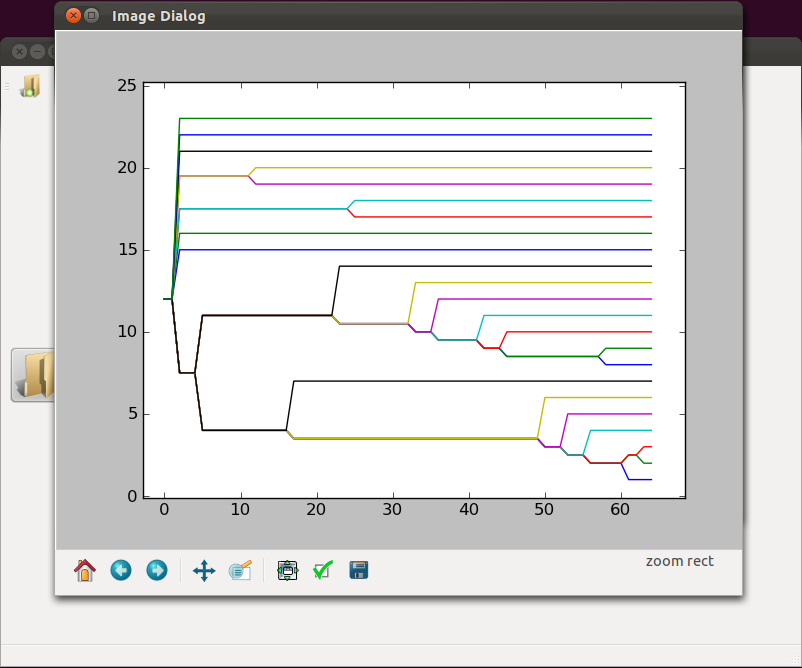
\includegraphics[scale=0.38]{navi-dendrogram}
\caption{Dendrograma mostrado pelo AIAF.}
\label{fig:navi-dendrogram}
\end{figure}

\section{Dificuldades} \label{sec:dificuldades}

Uma das principais dificuldades, sem dúvida, foi conseguir pensar em um sistema que pudesse ser ao mesmo tempo extensível, garantisse uma facilidade de uso,
se mostrasse rápido, de fácil manutenção, seguindo as boas práticas de modelagem e programação, sem perder a integração com o código legado. Tais
características exigiram um pensamento integrado na modelagem, implementação e processo de desenvolvimento, sem fugir aos requisitos e aos interesses dos dois
grupos de usuários: os pesquisadores e os desenvolvedores.

Ao longo do trabalho, houve complicações nas decisões de projeto e na modelagem. Na parte da implementação, a migração de alguns códigos originalmente em Perl
para Python e a opção de abandonar um banco de dados relacional tomaram uma boa parte do tempo, como também o aprendizado de PyQt e o desenvolvimento da
interface gráfica.

Apesar das dificuldades e da não implementação de alguns casos de uso, a modelagem realizada e o desenvolvimento do protótipo dentro do modelo em espiral
consistiram um trabalho importante, cujas considerações finais estão dispostas no próximo Capítulo.